\subsection{Accelerometer}
Et accelerometer er en elektromekanisk enhed, som både kan måle statisk eller dynamisk accerleration. Den statiske acceleration kan være tyngdekraften, hvortil det er muligt at bestemme orienteringen af accelerometeret i forhold til jorden. De dynamiske kræfter såsom bevægelse, stød og vibrationer, gør det muligt at analysere accelerometeres bevægelse samt hastighed. 

I dette projekt anvendes accelerometeret ADXL335Z, som har pin konfigurationen, som kan ses på \autoref{fig:acc_pin}. Accelerometeret er en 3-aksialt sensor, som har et arbejdsområde på minimum $\pm$ 3 g, og et output som spænding. Det analoge output signal er proportionelle med accelerationen \citep{analogdevices2010}. 


\begin{figure}[H]
\centering
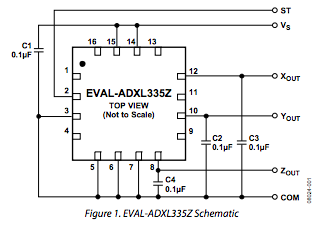
\includegraphics[width=1\textwidth]{figures/acc_pin.png}
\caption{Pin konfiguration af accelerometer ADXL335}
\label{fig:acc_pin}
\end{figure}

\noindent
Accelerometeret har en single-supply spændingsforsyning som ligger mellem 1,8 - 3,6 V, denne er reguleret til XX V via tilkobling af en regulator \fxnote{afhænger af hvad Jan sætter regulatoren til}. Offsettet er afhængig efter spændingsforsyningen, men ligger ved XX V på  XX V, denne beregnes som det halve af spændingsforsyningen. Båndbredden og støjen varierer for de forskellige akser. For x og y-aksen ligger båndbredden mellem 0,5 til 1.600 Hz og støjen normalt på 150$\mu g/\sqrt{Hz}$ RMS, mens båndbredden for z-aksen ligger mellem 0,5 til 550 Hz og støjen normalt på $300\mu g/\sqrt{Hz}$ RMS.  \fxnote{Den spektrale effekttæthed måles i $\mu g/$ og dividere dette med kvadratroden for båndbredden for signalet $\sqrt{Hz}$, hvilket giver RMS af accelerationsstøjen ved en temperatur på $25^\circ$C}. 

Da accelerometeret er ratiometrisk, hvilket vil sige at outputtet er direkte propotienelt med input, afhænger sensitiviteten ligesom offsettet af spændingsforsyningen. Ved XX V spændingsforsyning, ligger forsyningen på XX mV/g med en tolerance på XX \%, hvor outputimpedansen er XX k$\omega$ med en afvigelse på xx \%. 

\begin{figure}[H]
\centering
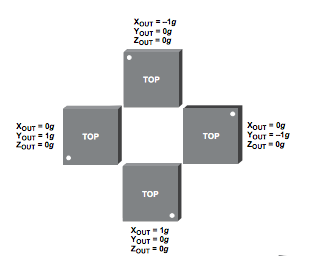
\includegraphics[width=1\textwidth]{figures/acc.png}
\caption{Accelerometeret, ADXL335z, påvirkning i de forskellige akser}
\label{fig:acc}
\end{figure}

\noindent
Accelerometeret hældes til siden, vil der ske en acceleration i forhold til tyngdekraften afhængig af, hvilken retningen og plan det hældes i. Dette fremgår af \autoref{fig:acc}. Herved vil der ske en ændring i spændingen fra referencepunkt ved en hældning på 0 $^{\circ}$. Hvis accelerometeret eksempelvis befinder sig i den øverste situation på \autoref{fig:acc}, påvirkes x-aksen med -1 g. Denne sammenhæng og derved patientens hældning kan udtrykkes ved følgende ligning:

\begin{equation}
	V_{out} = V_{offset} + sensitiviteten \cdot \sin(vinklen) \\
\end{equation}


%Støj kan reduceres ved at placere en 0.1 mikro f capacitor i nærheden, det er dog nødvendigt at tilføje mere, hvis der er 50 KHz støj, da det vil kunne resultere i fejl i accelerations målingen. Støjens tæthed vil forminskes i takt med at forsyningsspændingen forøges.
%Fase sensitiv demodulation teknikker er anvendt for at bestemme magnituden samt accelerationens retning. Demodulator outputtet er forstærket og bragt igennem en 32 k ohm modstand. – noget med det forebygger aliasing 
%  - Jeg ser dette som 'ligegyldigt' nu, da det handler om kondensator og støj. Kan ikke se hvorfor det skal bruges (endnu) måske skal det bruges efter vi har lavet pilotforsøg, hvis der viser sig meget støj